\chapter{Theory}
\label{sec:theory}

\section{Design Load Cases}
The user must specify the metocean conditions that drive the wind and
wave loads upon the floating substructure.  Ideally, multiple metocean
conditions would be used for design optimization.  This includes
standard operating conditions that determine fatigue loads, maximum
allowable operating conditions (e.g. max thrust), maximum survivable
conditions even if the rotor blades are parked, and likely others that
bound a design.  As of this writing, \textit{FloatingSE} only supports
execution and optimization around a single metocean condition and load
case.  Future development will enable optimization against multiple load
cases, likely those used in code standards.

\section{Load Path}
Similar to the assumptions in \textit{JacketSE}, as stated by
\citep{JacketSE}, the primary simplification in \textit{FloatingSE} is
the treatment of all loads as pseudo-static. This approximation reduces
computational time and resources, as an accurate calculation of dynamic
loads requires more sophisticated numerical tools and simulations.
Thus, users must exercise care in selecting loads and safety factors to
compensate for the lack of a fully dynamic treatment.  Furthermore,
fatigue effects and structural lifetime estimates are also not currently
calculated, but could be incorporated in future developments.  In
general though, fatigue loading tends to dominate the design of joints,
flanges, and welds in a design, whereas the main shell geometry is
driven by modal and buckling-strength requirements.

A floating wind turbine undergoes loading from a number of sources.  The
primary loading source for the tower comes from the aerodynamic loads
induced by the rotor. The substructure must resist the combination of
rotor loads and hydrodynamics loads, with the latter becoming more and
more important as water depth and wave heights increase.  Self-loading
from gravity acting on components is also accounted for. Other sources
of loading, such as installation loads, accidental loads, vortex-induced
vibrations, ice, and seismic loads are ignored.

Some of the included loads are calculated within \textit{FloatingSE} and
some are calculated in other WISDEM modules.  Wind and wave loads are
computed here.  Rotor thrust loads are computed in \textit{RotorSE}, and
imputed into \textit{FloatingSE} as inputs.  Loading over the entire
turbine is assembled within \textit{FloatinSE} for a structural analysis
via Frame3DD (via \textit{pyFrame3DD}).  Once all member loads and
stresses are determined, compliance checks against international
standards are evaluated and can be used as design constraints during
optimization runs.

\subsection{Wind and Wave Loads}
Wind drag loads are applied to the tower body and the upper part of the
substructure that extends above the waterline.  They are not applied to
connecting truss members that may be part of the substructure geometry.
These drag loads are
computed assuming the tower and columns are smooth circular
cross-sections and that the drag coefficient can be selected as a
function of the flow Reynolds number \citep{Roshko}.  The calculations
of the wind and wave loads are provided by multiple modules within
\textit{CommonSE}.

For the tower and portion of the substructure that extends above the
waterline, wind loading arises from the aerodynamic drag on the
structure.  This drag changes with height, since the wind profile
varies.  WISDEM allows the user to select from a power-law or
logarithmic scaling of wind with height, where the power-law
approximation is given by,
\[
  U_a(z) = U_{ref}\left(\frac{z}{z_{ref}}\right)^{\alpha}
\]
where $U(z)$ is the velocity as a function of height, $U_{ref}$ is a
reference wind speed measured at a reference height, $z_{ref}$, and
$\alpha$ is the shear exponent used in the power-law approximation of
wind profiles.

The wind aerodynamic drag, Reynolds number (and drag coefficient) are
allowed to vary as a function of height, according to the wind velocity
distribution,
\begin{equation} \label{eqn:drag}
  dF(z) = \frac{1}{2} \rho_a U_a^2(z) d(z) c_d(Re) dz;\qquad
  Re_d = \frac{\rho_a U_a(z) d(z)}{\mu_a},
\end{equation}
where $Re_d$ is the Reynolds number based on diameter, $\rho_a$ and
$\mu_a$ are the density and viscosity of air, $d(z)$ is the diameter of
the tower as a function of height, $c_d$ is the drag coefficient, and
$dF(z)$ is the force per unit length in the z-direction.

Wave drag loads arise from similar processes, but are computed using
Morison's equation to account for the different fluid properties
relative to air.  Wave particle velocity (not the same as the bulk
velocity of the wave) is assumed to follow linear (Airy) wave theory
\begin{equation} \label{eqn:Uwave}
U_w(z) = a\omega\frac{\cosh\left[\kappa\left(z + D \right)\right]}{\sinh\left(\kappa D\right)}\cosh\left(\kappa x -
  \omega t\right);
\qquad \omega=\frac{2\pi}{T} = \sqrt{ g \kappa \tanh\left(\kappa D\right) }
\end{equation}
where $\omega$ is the circular frequency, $T$ is the wave period, $a$ is
the wave amplitude (half of the significant wave height), $D$ is the total water depth, $g$ is the
acceleration of gravity, and $\kappa$ is the
wave number computed from the dispersion relationship given as the last
expression in Equation \ref{eqn:Uwave}.  Note that the horizontal
particle velocity varies in time and space (by the $\kappa x - \omega
t$) term.  Thus, the individual particles in the wave are also
accelerating at different rates,
\begin{equation} \label{eqn:Awave}
\dot{U}_w(z) = a\omega^2\frac{\cosh\left[\kappa\left(z + D \right)\right]}{\sinh\left(\kappa D\right)}\sinh\left(\kappa x -
  \omega t\right)
\end{equation}
where $\dot{U}(z)$ is the acceleration as a function of height.  For
simplicity, \textit{FloatingSE} only considers the maximum velocity and
acceleration at a given height, and makes a conservative assumption that
they occur concurrently in time and space.  This essentially means ignoring the
$\kappa x - \omega t$ term, since the maximum of any $\cosh$ or $\sinh$
term is one.

Morison's equation is a semi-empirical expression, as opposed to a model
of a specific physical process, that predicts the total hydrodynamic
loads.  It is comprised of two components, one for viscous drag
contributions and another for inertial effects (which includes incident,
diffracted, and radiated wave effects).  For flow past structures with
circular cross sections, Morison's equation for force per unit length
($dF(z)$) takes the form,
\begin{equation} \label{eqn:morison}
  dF(z) = \frac{\pi d^2(z)}{4} \rho_w C_m \dot{U}_w(z)dz + \frac{1}{2} \rho_w U_w^2(z) d(z) c_d(Re)dz
\end{equation}
where $C_m$ is the added mass coefficient (assumed to be $C_m=2$),
$U_w(z)$ is the current speed as a function of height, and the Reynolds
number is computed by substituting in the appropriate properties for
water,
\[
Re_d = \frac{\rho_w U_w(z) d(z)}{\mu_w}
\]


\subsection{Rotor Nacelle Assembly (RNA) Loads}
From a quasi-steady-state point of view, the RNA loads reduce to three
forces and three moments along the main coordinate axes
\citet{JacketSE}. The thrust is the biggest force responsible for the
bending moment distribution along the tower and loads on the
substructure.  There is the additional effect of the gravitational load
caused by the offset of the RNA center of mass from the tower
centerline.  This effect is more pronounced for downwind turbines than
upwind turbines, but is included regardless.

\textit{FloatingSE} does not compute the force and moment components and
accepts them as inputs from other WISDEM modules or from the user
directly.  Therefore, the methodology and fidelity in the RNA loads
calculation is not addressed in this document.


\subsection{Loads Integration and Structural Analysis}
The analysis tool, Frame3DD, is an open-source tool for static and
dynamic structural analysis of 2-D and 3-D frames and trusses with
elastic and geometric stiffness. It computes the static deflections,
reactions, internal element forces, natural frequencies, and modal
shapes using direct stiffness and mass assembly \citep{frame3dd}.  The
WISDEM toolkit developed a python interface, \textit{pyFrame3DD}, to avoid the
use of intermediate input and output text files.

All of the loads integration happens within Frame3DD, where the whole
floating turbine load path, from the rotor to the keel of the
substructure, is modeled with simple Timoshenko frame elements.  The
forces, moments, and mass properties of the rotor-nacelle assembly (RNA)
are inputs to \textit{FloatingSE} (mass properties are assumed to be
relative to the tower top position).  It assumed that the RNA is a rigid
body with respect to the tower modes and the mass properties, forces,
and moments, are applied to the corresponding node in the model.  Long
slender components, such as the tower and substructure columns, are
broken up into a finer discretization than the physical ``cans'' that
they are actually made of.  This finer discretization gives greater
resolution of internal forces and natural frequencies.  The wind and
wave forces per unit length in Equations \ref{eqn:drag} and
\ref{eqn:morison} are applied as trapezoidally varying loads along the
column elements.  Substructure pontoons are represented as single frame
elements.  Rigid boundary conditions for all 6 degrees of freedom (DOF)
are imposed at the windward mooring line connection, which is assumed to
be aligned with the wind, wave, and rotor thrust loads.  Aside from the
RNA, wind, and wave loads, other loads applied to the structure include
the gravity loads, and the buoyancy acting on the submerged elements.

Frame elements are described by their cross sectional properties (area,
moments of inertia, modulus of elasticity, and mass density) and
starting and ending nodes.  For simple geometries, such as pontoons with
tubular cross sections, these properties are straightforward
calculations.  For the turbine tower, tubular cross section properties
are also used, albeit at a finer discretization.  For substructure
columns, which may have permanent or variable ballast and bulkheads,
it is assumed that these extra features are not load-bearing, so
tubular cross section properties are also used.  However, the material mass
density of the frame element is scaled to reflect the true mass of the
whole section, including ballast, to ensure that gravity loads are
captured correctly.  Thus, for the tower,
columns, and pontoons, only cylindrical (tubular) cross-sections are
supported for now.  Future development may support other cross-sectional
geometries.  For the tubular cross sections, the critical properties needed by
Frame3DD are,
\begin{align*}
  \textrm{Outer radius, } r_o &= d/2\\
  \textrm{Inner radius, } r_i &= r_o - t\\
  \textrm{Material area, } A &= \pi \left( r_o^2 - r_i^2 \right)\\
  \textrm{Bending second moment of area, } I_{xx} &= I_{yy} = \frac{\pi}{4}\left( r_o^4 - r_i^4 \right)\\
  \textrm{Torsion second moment of area, } I_{zz} &= J_0 = I_{xx} + I_{yy}\\
  \textrm{Shear area, } A_{s} &= A / \left[ 1.124235 + 0.055610\left(\frac{r_i}{r_o}\right) +
           1.097134\left(\frac{r_i}{r_o}\right)^2 - 0.630057\left(\frac{r_i}{r_o}\right)^3 \right]\\
  \textrm{Bending modulus, } S &= I_{xx} / r_o \\
  \textrm{Torsion modulus (shear constant), } C &= I_{zz} / r_o
\end{align*}
where $d$ is the tube diameter and $t$ is the tube (or wall) thickness,
which are the common design variables for the tower, columns, and
pontoons. Note that the shear area expression is an empirical relationship as
opposed to an analytical expression.

\begin{figure}
  \begin{center}
    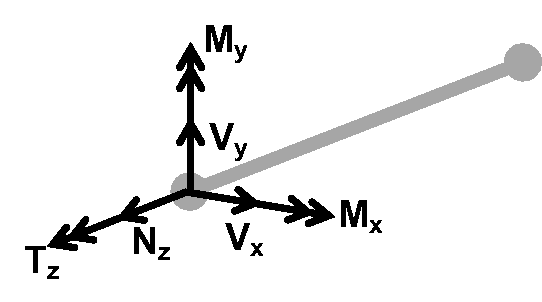
\includegraphics[width=2in]{figs/frameCS.pdf}
    \caption{Coordinate system for frame element forces.}
    \label{fig:frameCS}
  \end{center}
\end{figure}

Simulation outputs include mass properties of the structure, member
stresses, and summary forces and moments on the body.  Mass properties
include the total mass of the floating turbine and the mass of the
substructure itself.  The calculations also allow for easy computation
of the center of mass of the structure, not accounting for variable
ballast which is computed elsewhere, and the center of buoyancy
(centroid of the submerged volume).  The first two natural frequencies
of the structure are also computed to compare against the rotor passing
frequencies (1P and 3P).  Next, the reaction forces and moments at the
boundary mooring load are taken as the total loading on the structure.
These are used later in the static stability calculations to ensure that
the mooring lines provide adequate restoring force and moment.  Finally,
the axial and shear forces are extracted and converted
to stresses using cross-section properties for all elements.  These
element member loads follow the sign convention in Figure
\ref{fig:frameCS},
\begin{align*}
  \sigma_z &= \frac{N_z}{A} - \frac{\sqrt{M_x^2 + M_y^2}}{S}\\
  \tau_{z\theta} &= \frac{T_z}{C} + \frac{\sqrt{V_x^2 + V_y^2}}{A_s}
\end{align*}
where $N$ is the axial force (tension or compression), $T$ is the
torsional moment, $V$ is the shear force, $M$ is the bending moment,
$\sigma_z$ is the axial stress, and $\tau_{z\theta}$ is the shear
stress.  

Hoop
stress of the tower is estimated from the dynamic pressure of the
wind loads using the Eurocode method.  Hoop stress of the submerged
columns is determined using the dynamic and static pressure heads of the
water.
\begin{align*}
  \sigma_{\theta,Euro} &= k_w q_{max} \frac{d-t}{2t};\qquad q_{max} =
                         \frac{1}{2}\rho_a U_a^2\\
  \sigma_{\theta,hydro} &= \left(q_{max}+p_{hydro}\right) \frac{d-t}{2t};\qquad q_{max} =
                          \frac{1}{2}\rho_w U_w^2\\
  p_{hydro} &= \rho_w g \left( a\frac{\cosh\left[\kappa\left(z + D \right)\right]}{\cosh\left(\kappa D\right)} - z\right)
\end{align*}
where $\sigma_{\theta}$ is the hoop stress, $k_w$ is the TODO, $q_{max}$
is the maximum dynamic pressure on a cross-section, and $p_{hydro}$ is
the hydrostatic pressure with contributions from wave motion and the
static head.  Note that argument, $(z)$, was dropped without losing generality.

All stress components are combined into a von Mises stress for
comparison against a yield criterion,
\[
  \sigma_{vm} = \sqrt{\sigma_z^2 + \sigma_{\theta}^2 -
    \sigma_z\sigma_{\theta} + 3\tau_{z\theta}^2}
\]
where $\sigma_{vm}$ is the von Mises stress and $\sigma_{theta}$ is chosen
as the relevant hoop stress.  The von Mises stress is compared against
the yield stress, $\sigma_y$, and a safety factor as utilization criterion.


\subsection{Code Compliance as Utilizations}
Once the stress components of all structural members are computed, they
are compared against design code standards for compliance.
These standards serve as design constraints when conducting optimization.

Differing code standards are used for different components.  The turbine
tower and substructure pontoons stress components (axial, shear, and
hoop) are evaluated against a von Mises yield criterion with an
allowance for a margin of safety.  Tower segment stresses and geometry
are also evaluated against a shell buckling criterion published by
\citet{Eurocode} and a global buckling criterion \citet{Germanischer}.
Note that the implementation of the Eurocode buckling is modified
slightly so as to produce continuously differentiable output.  See
\citet{JacketSE} for a more detailed exposition.

The buckling criterion applied to the tower is not suitable for the
submerged columns of a spar or semisubmersible substructure due to the
higher hydrostatic pressure loads and use of ring stiffeners.  For these
submerged columns, the code standards applied are from the
\citet{api2U}, Bulletin 2U (specifically the procedure outlined in
Appendix B).  These standards also apply shell and general buckling
criterion with a margin of safety.


\section{Static Stability}
\label{sec:static}
\subsection{Neutral Buoyancy}
Any floating body requires enough water displacement to create
sufficient buoyancy force such that the body stays afloat in the most
extreme loading and environmental conditions.  This level of
displacement would otherwise be overkill for more benign loading
conditions.  Since a floating turbine is designed for a constant hub
height, variable amounts of ballast are required to maintain a neutrally
buoyant system for all operating conditions.  The variable ballast is
simply ocean water that is pulled in or pumped out of holding areas
within the substructure columns.

In \textit{FloatingSE}, the variable ballast water mass is calculated as the
difference between the total mass of displaced water and the total mass
of the floating turbine.  This mass is then divided by the water density
to obtain the variable ballast volume, which is then compared to the
frustum shell cross section profile above the permanent ballast to
determine the height of the water ballast within the column.  Once this
is determined, the final center of mass and center of buoyancy (centroid
of the submerged volume) of the
system can be determined.

\subsection{Surge/Sway Stability}
Surge and sway stability is not actively tracked over the coarse of a
load case.  Instead the total surge force on the structure is calculated
and compared to the restoring force of the mooring system at the maximum
allowable surge offset, which is specified by the user.  If the
restoring force at this maximum offset is greater than the surge force
applied, then the system is considered stable in surge.  Since the wind
and wave profiles are essentially 2-D in the $x-z$ plane, there are no
sway forces in the model.  Thus, sway stability is given the same
status as surge stability.

The surge direction is assumed to be aligned with the wind vector, which
is aligned with the $x$-axis.  Since the rotor yaw is assumed to be
$0^{\circ}$, the surge forces on the turbine include the rotor thrust,
the wind drag on the tower, and the wind and wave drag on the
substructure.  The final surge force over the whole structure is taken
from the $x$-direction reaction force of the windward reaction node in
the turbine-level Frame3DD analysis.  The total surge force on the
structure is only calculated at the initial conditions
(zero-displacement point), and not at the maximum offset condition.

The restoring force is calculated as the smallest possible restoring
force after a displacement in any angular direction in the mooring
model.  Since the alignment of the mooring lines relative to the
incoming wind direction is arbitrary, a maximum offset is simulated at
$2^{\circ}$ increments around the unit circle,
\[
  F_{x,restore} = \min_{i\in a} F_{x,i}\,;\qquad a= \left\{0^{\circ},
    2^{\circ}\ldots 360^{\circ}\right\}
\]
where $F_x$ is the surge force.  The smallest restoring force is used for the surge stability
calculations.  Also recorded is the maximum mooring line tension in any
line, in any direction, for comparison against the minimum breaking load
value,
\[
  T_{moor} = \max_{l\in L,i\in a} T_{l,i}\,;\qquad L=\left\{1,2\ldots
    nlines\right\}, \, a= \left\{0^{\circ}, 2^{\circ}\ldots 360^{\circ}\right\}
\]

\subsection{Pitch Stability}
The approach to pitch stability determination is similar to that of
surge stability.  The total pitching moment on the floating turbine is
calculated and compared to the restoring moment at the maximum allowable
angle of heel.  If the restoring moment at this max heel angle is
greater than the pitching moment applied, the system is said to be
statically stable in pitch.

Similar to the surge force calculation, the total pitching moment is
determined from the reaction moment at the windward boundary condition
in the Frame3DD analysis.  The pitching moment has contributions from
the wind and wave loads on the structure, the rotor forces and torques,
the buoyancy forces on the submerged substructure, and the off-center
weight of components (e.g. the RNA).  The total pitching moment is only
calculated at the $0^{\circ}$ pitch point, and not at the maximum heel
angle condition.

The restoring pitching moment has two primary contributions.  The first
is from the mooring lines.  Similar to the surge force calculation, here
the floating turbine is deflected in pitch by the maximum allowable heel
angle and the mooring forces are recorded.  Within the mooring
calculation, the center of mass of the turbine is not yet known, so the line
forces are saved in the simulation until that point is computed.  Then,
the restoring moment contribution from the mooring system is computed as,
\[
  \mbf{M_{moor}} = \sum_i \mbf{r_{cm-l}} \times \mbf{F_l}
\]
where $r_{cm-l}$ is the vector from the center of mass to the mooring
connection, $l$, and $F_l$ is the force applied by the $l$\th mooring
line.  As above, $F_l$ is taken as the minimum set over the possible
orientations of the mooring lines relative to the windward direction.

\begin{figure}
  \begin{subfigure}[b]{0.29\linewidth}
    \centering 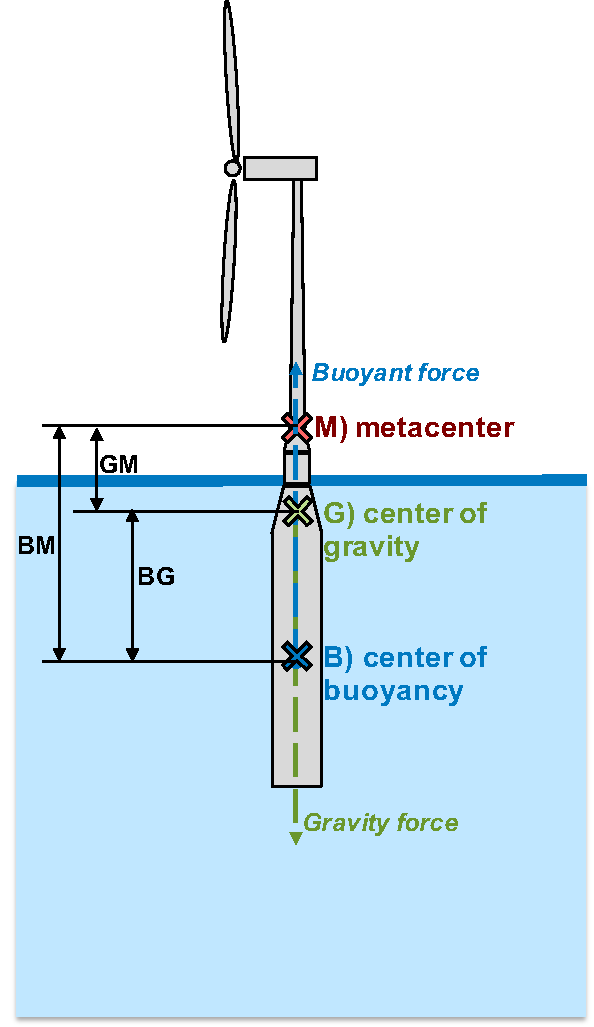
\includegraphics[height=3.25in]{figs/metacenterA.pdf}
    \caption{}
  \end{subfigure}
  \begin{subfigure}[b]{0.29\linewidth}
    \centering 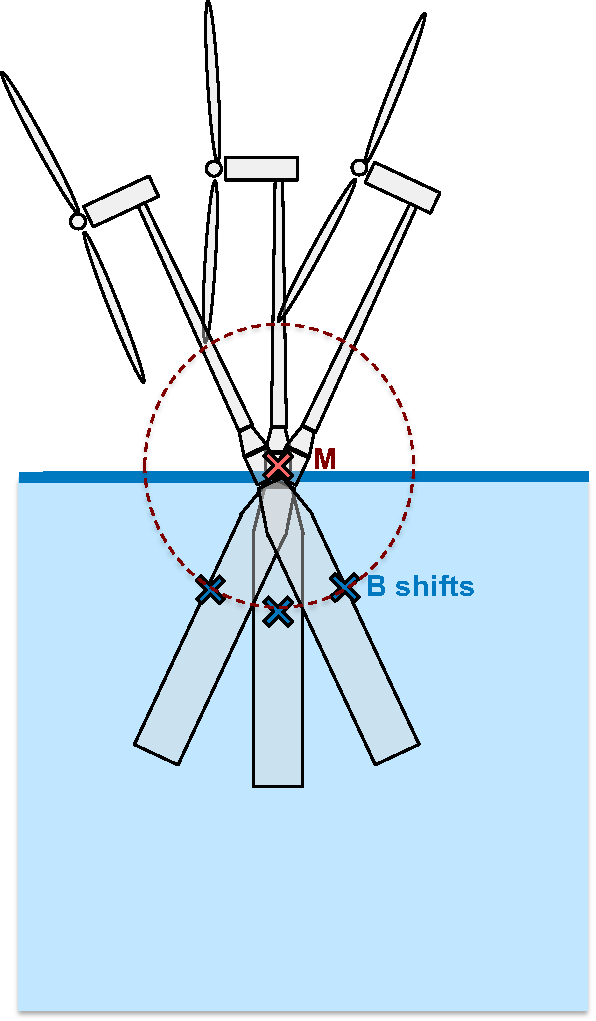
\includegraphics[height=3.25in]{figs/metacenterC.pdf}
    \caption{}
  \end{subfigure}
  \begin{subfigure}[b]{0.4\linewidth}
    \centering 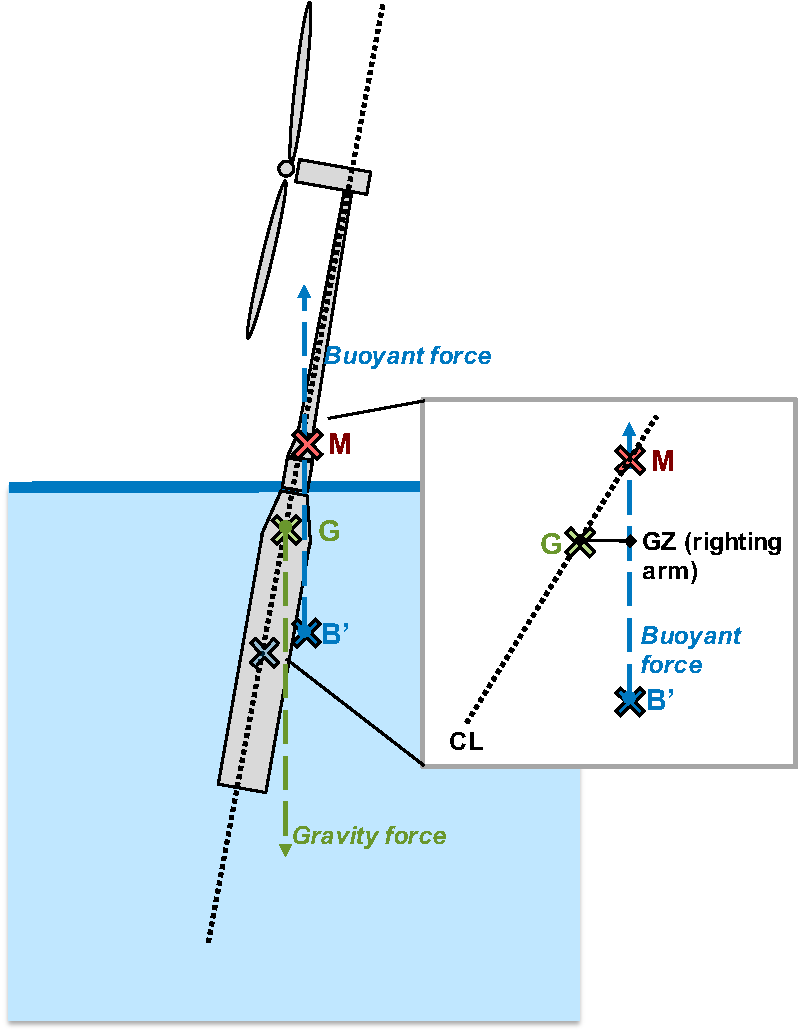
\includegraphics[height=3.25in]{figs/metacenterD.pdf}
    \caption{}
  \end{subfigure}\\
  \caption{Static stability of floating offshore wind turbines.}
  \label{fig:metacenter}
\end{figure}

The second contributing restoring moment comes from the motion of the
center of buoyancy away from alignment with the center of mass.  This is
a standard calculation in naval architecture \citep{thiagarajan2014} and is
diagrammed in Figure \ref{fig:metacenter}.  In this diagram, the center
of mass is denoted, $G$, the center of buoyancy is $B$, and the
metacenter is $M$.  In neural conditions (Figure \ref{fig:metacenter}a),
all of this points are vertically aligned.  The metacenter is defined as
the common point through which the buoyancy force acts as it pitches
through small displacements (Figure \ref{fig:metacenter}b), for bodies
with sufficient freeboard margin.  The metacenter point is most easily
calculated as an offset from the center of buoyancy ($BM$) by,
\[
  BM = \frac{I_w}{V}
\]
where $I_w$ is the second moment of area of the substructure waterplane
(with units of \unit{$m^4$}) and $V$ is the total volume of displacement
(with units of \unit{$m^3$}).  Note that for semisubmersible type
geometries, $I_w$ is calculated with the parallel axis theorem for all
of the columns at the waterplane,
\[
  I_w = \sum_i \left( I_{w,i} + A_{w,i}r_i^2 \right)
\]
where $A_w$ is the cross sectional area of the $i$\th column and $r_i$
is the distance from the waterplane centroid to the $i$\th column centroid.

As the structure lists or heels, the center of buoyancy shifts toward
the side of the structure that is more submerged (from $B$ to $B'$) and
the buoyancy force no longer passes through the center of mass.
Instead, the buoyancy force passes through the metacenter (by its
definition) with an effective moment arm of $GZ$ from the center of mass
(Figure \ref{fig:metacenter}c).  By geometry,
\[
GZ = GM \sin \theta
\]
where $\theta$ is the angle of heel.  The restoring moment is then the
buoyancy force acting through the restoring arm, $GZ$,
\[
  M_{meta} = F_B \left(GZ\right)
\]
For this reason, the metacenter must be located above the center of mass
for static stability.  This condition is imposed on the design as an
optimization constraint.  Note that the total volume of displacement,
and the subsequent buoyancy force, is not recalculated in the perturbed
configuration.  It is assumed that the angles of deflection are small
and that there is sufficient freeboard and design symmetry such that the
total displacement is constant.

The total restoring pitching moment is then the sum of these two
contributions,
\[
  M_{y,restore} = M_{y,moor} + M_{meta}
\]

\subsection{Heave, Roll, Yaw Stability}
The heave, roll, and yaw degrees of freedom are not yet modeled in
\textit{FloatingSE}.  Future improvements to the module will consider adding
these features.

\section{Mooring Lines}
The steady-state mooring system analysis is handled by the external Mooring Analysis
Program (MAP++) library \citep{MAP}, which has convenient Python bindings
to access the simulation output.  From its website
(\url{https://nwtc.nrel.gov/MAP}),
\begin{quote}
  \textit{MAP is designed to be used in parallel with other tools to model the
  steady-state forces on a Multi-Segmented, Quasi-Static (MSQS) mooring
  line. The MSQS model is developed based on an extension of
  conventional single line static solutions. Conceptually, MAP++'s MSQS
  module solves the algebraic equations for all elements simultaneously
  with the condition that the total force at connection points sum to
  zero. Seabed contact, seabed friction, and externally applied forces
  can be modeled with this tool. This allows multi-element mooring lines
  with arbitrary connection configurations to be analyzed.}
\end{quote}

MAP++ inputs are passed through a text-file, and include sea depth, geometry
descriptions of the mooring line connections, and material properties of
the lines.  For chain and rope-based cables, these material properties
are not easily derived and would be typically provided by a
manufacturer.  We borrow from the approach of the popular Orcina OrcaFlex
software \citep{orca} and use the following expressions,
\begin{align*}
MBL &= 2.74\times 10^7  D^2 \left(44 - 80D\right) \unit{N} \\
mass &= 19.9\times 10^3 D^2 \unit{kg/m}\\
A &= 2\left(\pi D^2 / 4 \right)\\
EA &= 0.854e11 D^2\unit{m^2}\\
cost &= 3.415\times 10^4 D^2 \unit{USD}
\end{align*}
where $MBL$ is minimum breaking load, $D$ is the diameter of a single
half-chain link, $A$ is the chain cross-sectional area, $E$ is the
Young's modulus, $EA$ is the axial stiffness.  When conducting
optimization, the expression for $MBL$ is poorly posed due to its limited
range of diameter applicability, so a linear fit is used instead,
\[
MBL = 1000 \max\left(1.0, -5445.3 + 176972.7 D\right)
\]  

\section{Verification and Validation}
At the time of this writing, \textit{FloatingSE} has not yet been
subjected to a verification campaign.  This is planned in the near
future where estimates of mass properties and structural loading from
\textit{FloatingSE} will be compared to higher-fidelity tools such as
OpenFAST and Ansys.  Validation, where model results are compared to
experimental results, are not currently planned at this time.
